\chapter{Observables que conmutan, fases de energía y precesión del espín}

\lectureoverview{Comenzamos con el significado cualitativo de la incertidumbre. Dos observables solo pueden tener valores definidos simultáneamente si poseen una base completa común de autovectores, lo que equivale a que sus operadores conmuten. Después repasamos la evolución unitaria y la ecuación de Schr\"odinger, comparamos los conmutadores con los corchetes de Poisson clásicos, resolvemos la ecuación dependiente del tiempo en la base de energía y aplicamos el resultado al espín en un campo magnético. El cálculo final da la precesión de los valores esperados del espín, los dos niveles de energía de un Hamiltoniano general para el espín y la distinción entre un valor esperado transversal y un fotón con la mitad de la diferencia de energía.}

El espín de dos estados sigue siendo nuestro sistema cuántico más sencillo. Un espacio de Hilbert de tres estados sería la siguiente posibilidad abstracta más sencilla; dos espines ya tienen cuatro estados de base ortogonales. Todavía no compondrán dos espines, aunque ese paso está cerca y traerá consigo el entrelazamiento. Primero debemos terminar el problema de un solo espín y asentar mejor las ideas de incertidumbre y evolución temporal.

\section{Cuándo pueden estar definidas simultáneamente dos cantidades}

Una buena medición es repetible. Si se mide un observable y se obtiene el valor \(l\), una repetición inmediata debería dar el mismo valor. Por tanto, la primera medición debe dejar el sistema, al menos momentáneamente, en un autoestado del operador correspondiente:
\begin{equation}
L\ket{l}=l\ket{l}.
\end{equation}
Esta afirmación operacional basta para revelar el origen cualitativo de la incertidumbre.

Supongamos que dos observables \(L\) y \(M\) pueden medirse simultáneamente. Una medición conjunta debe dejar definidos ambos valores registrados. Por consiguiente, los posibles estados posteriores a la medición deben ser autovectores simultáneos de ambos operadores. En el caso finito-dimensional que usamos aquí, podemos elegir un conjunto ortonormal completo \(\{\ket{i}\}\) que satisfaga
\begin{equation}
L\ket{i}=l_i\ket{i},
\qquad
M\ket{i}=m_i\ket{i}.
\label{eq:l5-common-eigenvectors}
\end{equation}

\begin{remark}
La palabra \emph{base} designará una base ortonormal completa. El álgebra lineal permite bases no ortogonales, pero la convención ortonormal resulta especialmente natural para los estados cuánticos. Los autovalores degenerados dejan libertad dentro de un autoespacio; en ese espacio, los autovectores pueden elegirse ortonormalmente.
\end{remark}

\begin{theorem}
Dos observables hermíticos de dimensión finita pueden medirse simultáneamente si y solo si admiten una base común completa de autovectores, lo que equivale a que conmuten.
\end{theorem}

La implicación directa se obtiene de inmediato a partir de la ecuación~\eqref{eq:l5-common-eigenvectors}. Si actuamos en un orden, resulta
\begin{align}
ML\ket{i}
&=M\bigl(l_i\ket{i}\bigr)\\
&=l_i m_i\ket{i},
\end{align}
mientras que en el orden inverso resulta
\begin{align}
LM\ket{i}
&=L\bigl(m_i\ket{i}\bigr)\\
&=m_i l_i\ket{i}.
\end{align}
Los autovalores son números ordinarios, de modo que \(l_i m_i=m_i l_i\). Así, \(ML\) y \(LM\) actúan de la misma manera sobre cada elemento de una base y, por tanto, sobre cualquier estado:
\begin{equation}
[L,M]\equiv LM-ML=0.
\label{eq:l5-commuting-condition}
\end{equation}

\begin{figure}[htbp]\centering
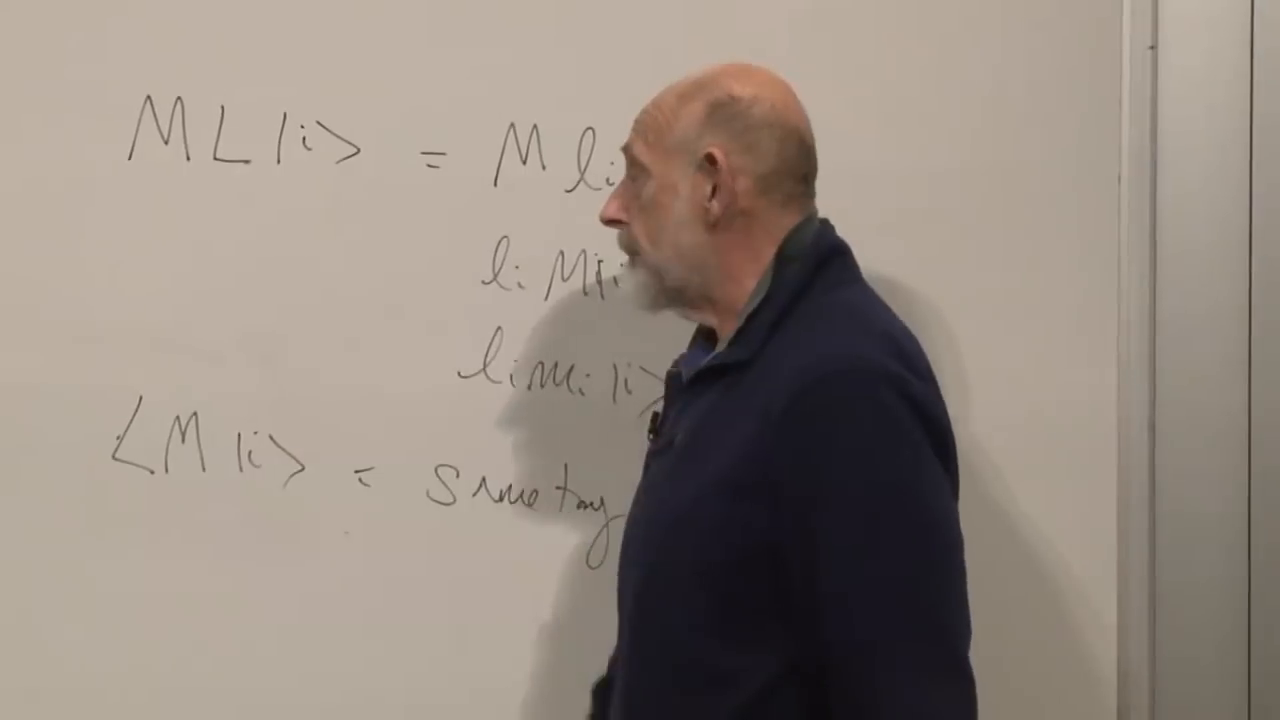
\includegraphics[width=0.86\textwidth]{lecture_05_figure_02.png}\caption{El argumento de los autovectores comunes lleva a \(LM-ML=[L,M]=0\).}\lectureframe{00:10:30}\end{figure}

También se cumple el recíproco: los operadores hermíticos que conmutan pueden diagonalizarse simultáneamente. Si un operador tiene un autoespacio degenerado, el otro lo conserva y puede diagonalizarse dentro de él. Al repetir este procedimiento en cada autoespacio se obtiene una base común completa de autovectores.

Los operadores de Pauli proporcionan el primer contraejemplo importante. Ningún par de \(\sigma_x,\sigma_y,\sigma_z\) conmuta. Los autoestados de \(\sigma_z\) son arriba y abajo, mientras que los de \(\sigma_x\) son derecha e izquierda. Se puede preparar con precisión cualquiera de las dos componentes y repetir su medición, pero no es posible preparar ambas componentes con precisión al mismo tiempo. Esta es la incertidumbre antes de introducir cualquier desigualdad numérica.

Más adelante cuantificaremos cómo las incertidumbres de dos observables que no conmutan se restringen mutuamente. Aquí no se demuestra ningún principio de incertidumbre numérico. La idea precede a la desigualdad: la falta de conmutación impide que un estado asigne valores definidos simultáneamente a ambas cantidades.

\begin{classroomqa}\audiencequestion{¿Por qué una medición simultánea requiere autovectores comunes?}\lecturerresponse{Una medición repetible deja un estado en el que el valor medido está definido, es decir, en un autoestado del operador medido. Si se obtienen dos valores a la vez y ambos siguen siendo repetibles, el estado resultante debe ser un autoestado de ambos operadores. Por tanto, el conjunto completo de resultados conjuntos proporciona una base común de autovectores.}\end{classroomqa}

\begin{classroomqa}\audiencequestion{¿Esto implica dos partículas distintas?}\lecturerresponse{No necesariamente: \(\sigma_x\) y \(\sigma_z\) ya actúan sobre un solo espín. Sin embargo, para dos subsistemas distintos, los observables que actúan sobre factores diferentes sí conmutan: \(A\otimes I\) conmuta con \(I\otimes B\). Por eso se pueden medir a la vez una componente de un espín y una componente de otro. Más adelante, al componer estos sistemas, aparecerá el entrelazamiento.}\end{classroomqa}

\section{Evolución unitaria y su generador}

La mecánica cuántica tardó bastante más que la mecánica clásica en definir un estado, pero, una vez establecido el espacio de estados, la regla del movimiento es concisa. Sea
\begin{equation}
\ket{\psi(t)}=U(t)\ket{\psi(0)}.
\label{eq:l5-propagator}
\end{equation}
La evolución temporal debe preservar la distinguibilidad. Más aún, preserva todos los productos internos. Para una base ortonormal,
\begin{equation}
\bra{j}U^\dagger(t)U(t)\ket{i}=\delta_{ji},
\end{equation}
y, por tanto,
\begin{equation}
U^\dagger(t)U(t)=I.
\label{eq:l5-unitarity}
\end{equation}
El operador de evolución es unitario.

En el tiempo transcurrido nulo, \(U(0)=I\). Por continuidad, la evolución durante un intervalo pequeño \(\epsilon\) difiere solo ligeramente de la identidad. En unidades donde \(\hbar=1\), escribimos
\begin{equation}
U(\epsilon)=I-i\epsilon H+O(\epsilon^2),
\qquad
U^\dagger(\epsilon)=I+i\epsilon H^\dagger+O(\epsilon^2).
\end{equation}
Al sustituir en la ecuación~\eqref{eq:l5-unitarity} se obtiene
\begin{equation}
H^\dagger=H.
\end{equation}
El generador de la evolución temporal es hermítico y, por tanto, un observable. Es el Hamiltoniano.

Al aplicar el propagador infinitesimal a un estado se obtiene
\begin{equation}
\ket{\psi(\epsilon)}
=\ket{\psi(0)}-i\epsilon H\ket{\psi(0)}+O(\epsilon^2).
\end{equation}
Al reorganizar la expresión se obtiene el cociente incremental que aparece en la pizarra:
\begin{equation}
\frac{\ket{\psi(\epsilon)}-\ket{\psi(0)}}{\epsilon}
=-iH\ket{\psi(0)}+O(\epsilon).
\end{equation}

\begin{figure}[htbp]\centering
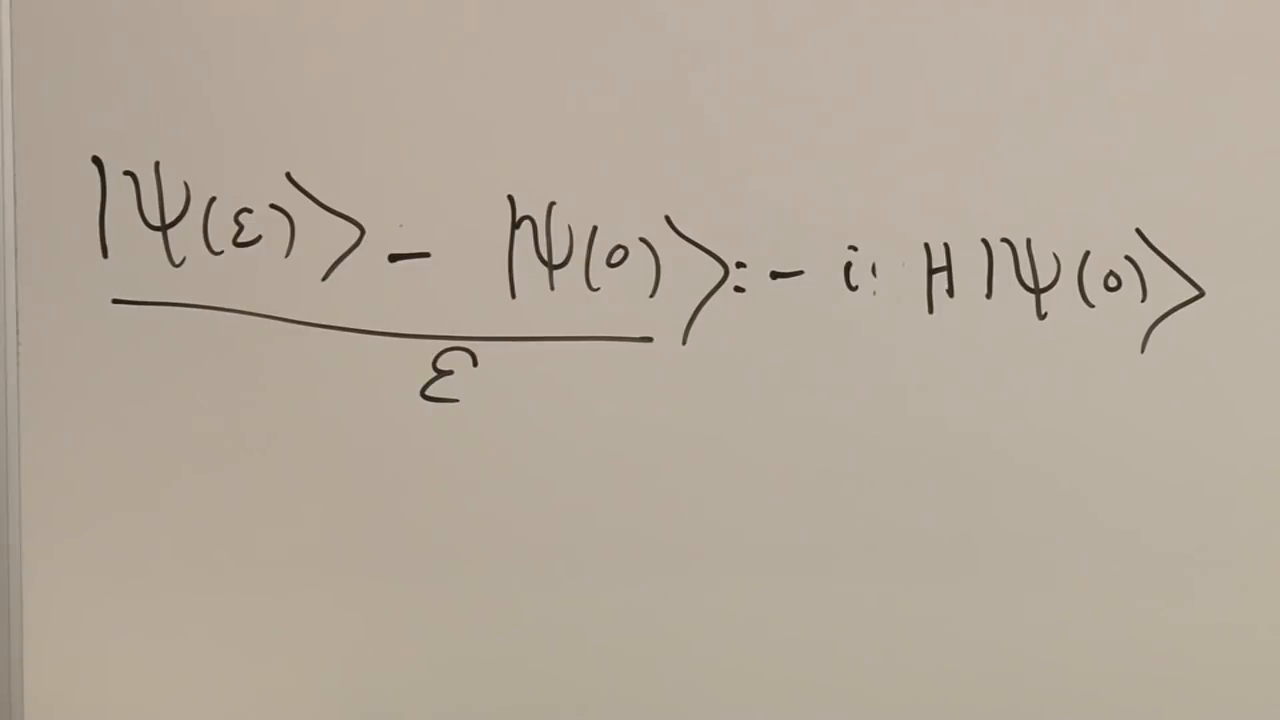
\includegraphics[width=0.86\textwidth]{lecture_05_figure_03.png}\caption{La actualización infinitesimal escrita como un cociente incremental.}\lectureframe{00:23:33}\end{figure}

Al tomar \(\epsilon\to0\) se obtiene la ecuación de Schr\"odinger dependiente del tiempo:
\begin{equation}
\frac{d}{dt}\ket{\psi(t)}=-iH\ket{\psi(t)}.
\label{eq:l5-schrodinger}
\end{equation}
Al restituir las constantes, esta es \(i\hbar\,d\ket{\psi}/dt=H\ket{\psi}\).

La ecuación original de Schr\"odinger se refería a la función de onda de una partícula en movimiento. A la formulación con operadores anterior se la llamó en su día ecuación de Schr\"odinger generalizada porque se aplica por igual a un espín, un sistema de tres estados, dos espines o un sistema de complejidad arbitraria. En gran medida se ha dejado de usar el adjetivo; hoy esta es simplemente la forma general de la ecuación.

La ecuación~\eqref{eq:l5-schrodinger} determina la evolución del estado cuando se deja el sistema sin perturbar. Esto no significa que todos los resultados experimentales estén definidos. Un estado cuántico determina las probabilidades de las mediciones posibles, y la ecuación actualiza esas probabilidades a través de los cambios de las amplitudes. En general, la medición cambia el estado e interrumpe esta evolución aislada.

\begin{classroomqa}\audiencequestion{¿Toda medición perturba el sistema?}\lecturerresponse{En general, sí, pero hay un caso especial importante. Si el estado ya es un autoestado del observable, una medición ideal y repetible puede confirmar su valor sin cambiar ese estado. Lo que, en general, no es posible es medir un observable arbitrario sin perturbar otras propiedades incompatibles.}\end{classroomqa}

\section{La energía y la ecuación independiente del tiempo}

Como \(H\) es hermítico, sus autovalores son reales y sus autovectores pueden elegirse como una base ortonormal completa:
\begin{equation}
H\ket{E_i}=E_i\ket{E_i}.
\label{eq:l5-time-independent}
\end{equation}
Esta es la forma independiente del tiempo de la ecuación de Schr\"odinger. Se trata de un problema de autovalores, no de una ecuación de movimiento: pregunta qué valores de energía puede tener el sistema y qué estados tienen esos valores definidos con precisión.

El espectro depende del sistema. El movimiento atómico ligado y el oscilador armónico tienen niveles de energía numerables. Una partícula no ligada puede tener un espectro continuo. La energía puede medirse de muchas maneras; en principio, incluso una medición de masa suficientemente precisa podría recurrir a \(E=mc^2\), aunque rara vez es el método práctico. Un sistema real ya tiene su Hamiltoniano; el físico no lo impone, sino que intenta descubrirlo. Una vez conocido ese operador, hallar sus autovalores y autovectores es la tarea matemática.

Añadir una constante \(cI\) a \(H\) desplaza todas las energías en \(c\). Multiplica el estado entero por una fase común \(e^{-ict}\), que no cambia las probabilidades ni los valores esperados. En la dinámica que consideramos aquí solo afectan las diferencias de energía.

\section{Cómo evolucionan los valores esperados}

La expresión habitual \emph{valor esperado} significa promedio estadístico. Para un observable \(L\),
\begin{equation}
\expect{L}(t)=\bra{\psi(t)}L\ket{\psi(t)}.
\end{equation}
En esta etapa, solo los vectores de estado dependen del tiempo. Al derivar ambos lados y usar la ecuación~\eqref{eq:l5-schrodinger} junto con su conjugada hermítica,
\begin{equation}
\frac{d}{dt}\ket{\psi}=-iH\ket{\psi},
\qquad
\frac{d}{dt}\bra{\psi}=i\bra{\psi}H,
\end{equation}
se obtiene
\begin{align}
\frac{d}{dt}\expect{L}
&=i\bra{\psi}HL\ket{\psi}
  -i\bra{\psi}LH\ket{\psi}\\
&=-i\expect{[L,H]}.
\label{eq:l5-expectation-motion}
\end{align}

\begin{figure}[htbp]\centering
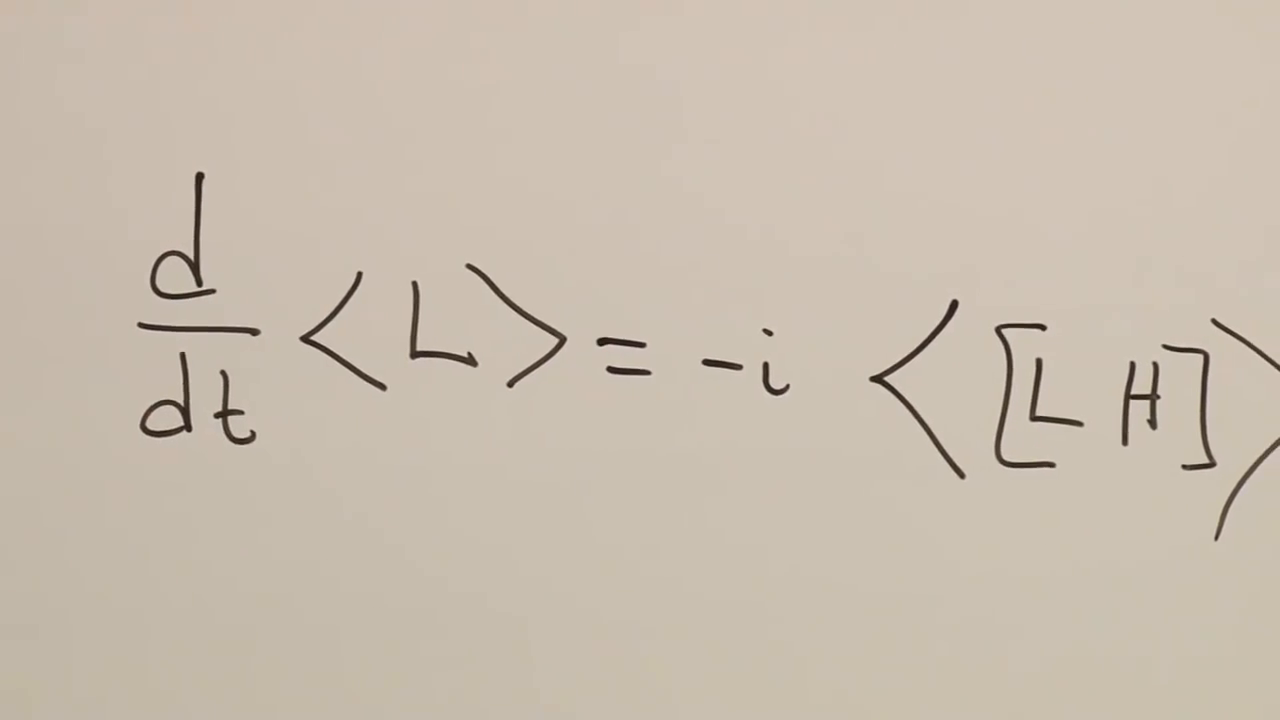
\includegraphics[width=0.86\textwidth]{lecture_05_figure_04.png}\caption{La ecuación de movimiento del valor esperado en forma de conmutador.}\lectureframe{00:35:35}\end{figure}

El factor \(i\) no pone en riesgo el carácter real de \(\expect{L}\). Para \(L\) y \(H\) hermíticos, el conmutador es antihermítico:
\begin{equation}
[L,H]^\dagger=-[L,H].
\end{equation}
Por tanto, su valor esperado es puramente imaginario, y al multiplicarlo por \(-i\) se obtiene una derivada real.

A veces se escribe la expresión abreviada
\begin{equation}
\dot L=-i[L,H].
\end{equation}
En este punto debe entenderse como una abreviatura de la ecuación~\eqref{eq:l5-expectation-motion}, una ecuación sobre promedios. Más adelante se introducirá un cambio completo de representación en el que los propios operadores dependerán del tiempo.

\subsection{El álgebra de los conmutadores}

Los conmutadores son antisimétricos:
\begin{equation}
[A,B]=-[B,A].
\end{equation}
También obedecen una regla del producto análoga a la regla de Leibniz para las derivadas:
\begin{equation}
[AB,C]=A[B,C]+[A,C]B.
\label{eq:l5-product-rule}
\end{equation}
Para comprobarlo, conservemos el orden de cada factor:
\begin{align}
A[B,C]+[A,C]B
&=A(BC-CB)\\
&\quad +(AC-CA)B\\
&=ABC-ACB\\
&\quad +ACB-CAB\\
&=ABC-CAB\\
&=[AB,C].
\end{align}

\begin{figure}[htbp]\centering
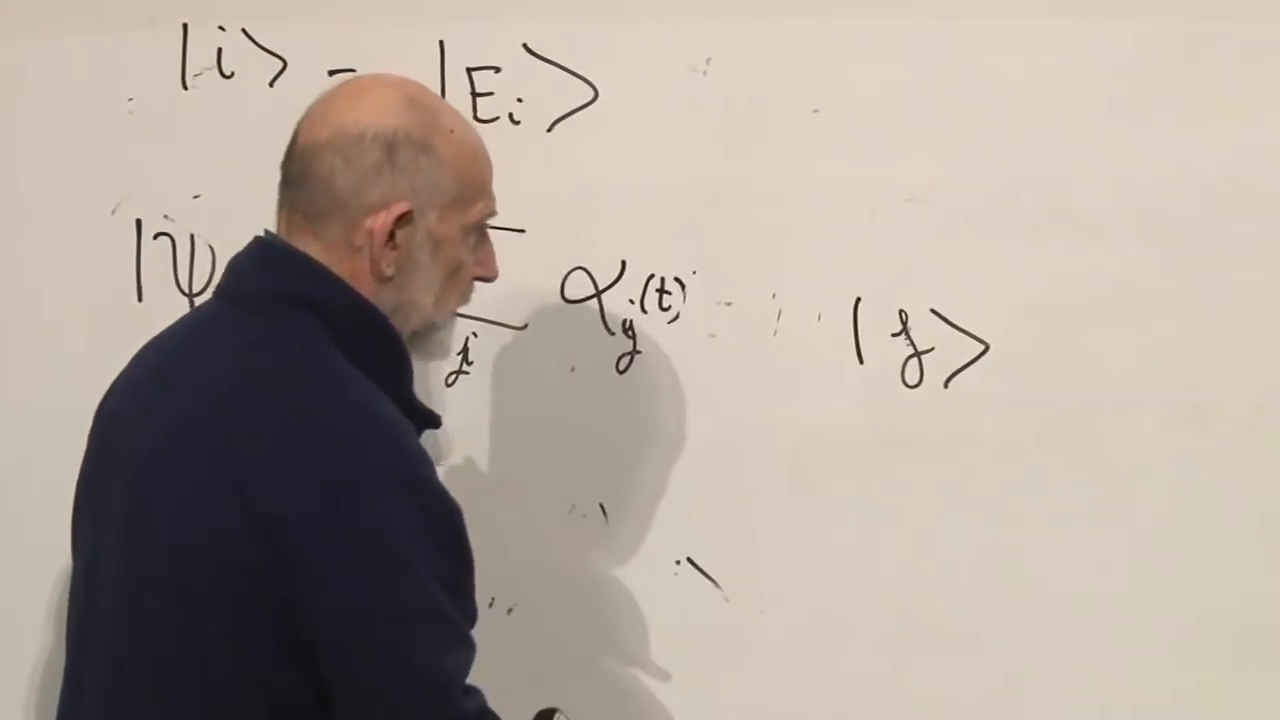
\includegraphics[width=0.86\textwidth]{lecture_05_figure_05.png}\caption{Comprobación de la regla del producto de los conmutadores al desarrollar ambos lados.}\lectureframe{00:43:10}\end{figure}

\begin{classroomqa}\audiencequestion{¿El lado derecho de la regla del producto cuenta por accidente dos veces el lado izquierdo?}\lecturerresponse{No. Al desarrollar la expresión, \(ABC\) y \(-CAB\) son los dos términos buscados. Los dos términos añadidos son \(-ACB\) y \(+ACB\), que se cancelan exactamente. La copia adicional aparente es el término provisional que hace falta para factorizar la expresión de las dos maneras requeridas.}\end{classroomqa}

La misma antisimetría y la misma regla del producto se cumplen para los corchetes de Poisson clásicos. Este parecido estructural no es casual. La correspondencia clásica es
\begin{equation}
\{A,B\}
\quad\longleftrightarrow\quad
\frac{1}{i\hbar}[A,B]
=-\frac{i}{\hbar}[A,B].
\label{eq:l5-poisson-correspondence}
\end{equation}
En unidades con \(\hbar=1\), la ecuación clásica
\begin{equation}
\frac{dL}{dt}=\{L,H\}
\end{equation}
tiene la misma forma que la ecuación~\eqref{eq:l5-expectation-motion}. En las unidades macroscópicas habituales, \(\hbar\) es pequeño, y los conmutadores se vuelven despreciables en el límite clásico apropiado. Esta es la comprobación esencial que identifica el generador cuántico \(H\) con el Hamiltoniano de la mecánica clásica.

El factor de \(\hbar\) es necesario por razones dimensionales. Un corchete de Poisson deriva respecto de coordenadas y momentos conjugados, mientras que un conmutador de operadores se construye directamente a partir de productos. La constante de Planck proporciona la conversión entre esas dimensiones.

Sea \(L=H\). Como todo operador conmuta consigo mismo,
\begin{equation}
\frac{d}{dt}\expect{H}
=-i\expect{[H,H]}=0.
\end{equation}
Para los Hamiltonianos independientes del tiempo que estamos considerando, el valor esperado de la energía se conserva. Es posible enunciar una afirmación más fuerte sobre la distribución completa de energía, pero aquí basta con el promedio.

\begin{classroomqa}\audiencequestion{¿Qué representa \(L\) en estas ecuaciones? ¿Es el momento angular?}\lecturerresponse{Aquí \(L\) es un operador lineal hermítico genérico y, por tanto, cualquier observable. Puede ser una componente del espín, una posición o incluso \(H\). Se eligió la letra por \emph{operador lineal} y no debe interpretarse como momento angular salvo que ese significado se especifique por separado.}\end{classroomqa}

\begin{classroomqa}\audiencequestion{¿Por qué el factor \(i\) no hace que un promedio real adquiera una derivada imaginaria?}\lecturerresponse{El conmutador de dos operadores hermíticos es antihermítico, así que su valor esperado es imaginario. El cálculo con matrices de Pauli que sigue lo muestra de manera concreta: sus conmutadores contienen un factor explícito \(2i\), que cancela el \(-i\) de la ecuación de movimiento.}\end{classroomqa}

\section{Resolución de la ecuación de Schr\"odinger en la base de energía}

Supongamos que se ha resuelto el problema de autovalores de energía. Desarrollemos un estado arbitrario en la base de energía fija:
\begin{equation}
\ket{\psi(t)}=\sum_j\alpha_j(t)\ket{E_j}.
\label{eq:l5-energy-expansion}
\end{equation}
En esta descripción, los vectores de la base no cambian; toda la dependencia temporal está en los coeficientes. Al sustituir la ecuación~\eqref{eq:l5-energy-expansion} en la ecuación~\eqref{eq:l5-schrodinger} se obtiene
\begin{align}
\sum_j\dot\alpha_j(t)\ket{E_j}
&=-i\sum_j\alpha_j(t)H\ket{E_j}\\
&=-i\sum_j E_j\alpha_j(t)\ket{E_j}.
\end{align}
La unicidad del desarrollo en una base implica, para cada \(j\) fijo,
\begin{equation}
\dot\alpha_j(t)=-iE_j\alpha_j(t),
\qquad\text{no sum on \(j\)}.
\end{equation}
La solución es
\begin{equation}
\alpha_j(t)=\alpha_j(0)e^{-iE_jt}.
\label{eq:l5-energy-phase}
\end{equation}

\begin{figure}[htbp]\centering
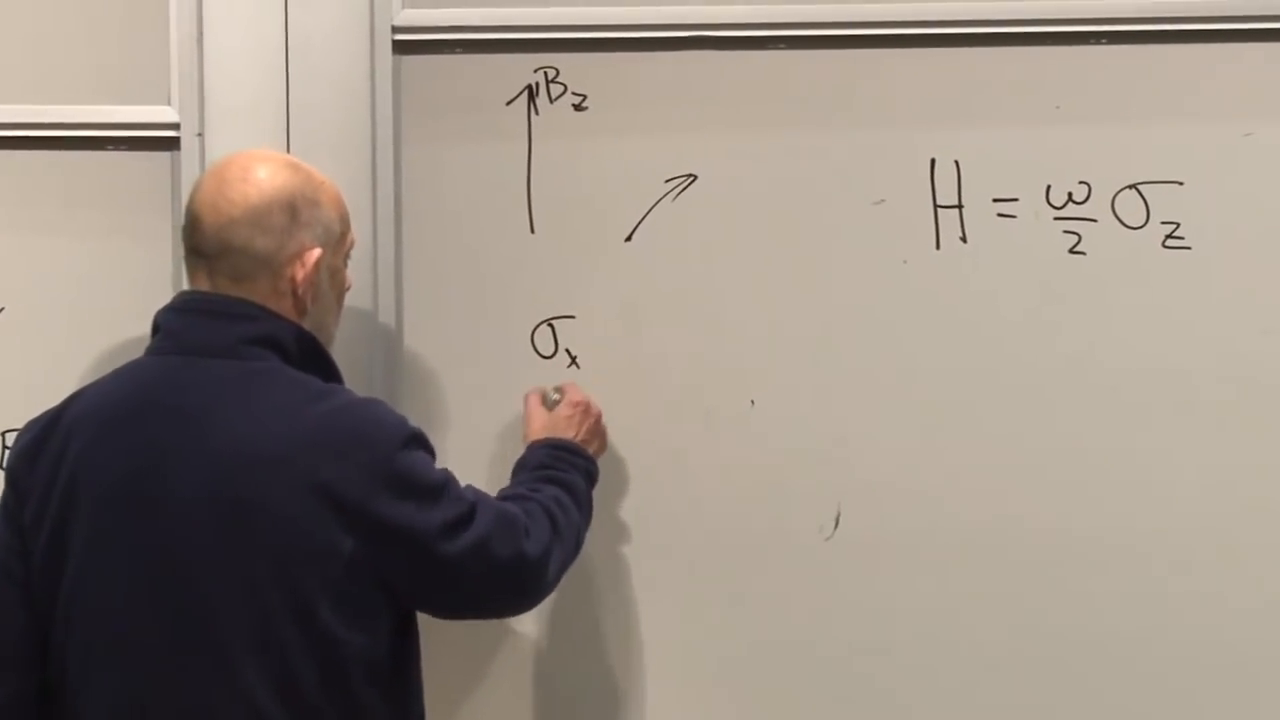
\includegraphics[width=0.86\textwidth]{lecture_05_figure_06.png}\caption{Cada coeficiente en la base de energía satisface su propia ecuación de fase exponencial.}\lectureframe{01:03:25}\end{figure}

Así, la solución general es
\begin{equation}
\ket{\psi(t)}
=\sum_j\alpha_j(0)e^{-iE_jt}\ket{E_j}.
\label{eq:l5-general-solution}
\end{equation}
Al restituir las unidades, se reemplaza \(E_jt\) por \(E_jt/\hbar\). El módulo de cada coeficiente permanece constante:
\begin{equation}
|\alpha_j(t)|=|\alpha_j(0)|.
\end{equation}
La evolución temporal cambia las fases relativas. Un único autoestado de energía adquiere solo una fase común y, por tanto, sus probabilidades de medición son independientes del tiempo.

Ahora podemos escribir explícitamente el valor esperado de \(L\). Definamos sus elementos de matriz en la base de energía mediante
\begin{equation}
L_{kj}=\bra{E_k}L\ket{E_j}.
\end{equation}
Entonces
\begin{align}
\expect{L}(t)
&=\sum_{k,j}
\alpha_k^*(0)\alpha_j(0)
e^{i(E_k-E_j)t}
L_{kj}.
\label{eq:l5-heisenberg-matrix}
\end{align}

\begin{figure}[htbp]\centering
\includegraphics[width=0.86\textwidth]{lecture_05_figure_07.png}\caption{La fórmula matricial en la base de energía: cada elemento lleva una fase con frecuencia de transición.}\lectureframe{01:10:45}\end{figure}

Los términos diagonales \(k=j\) son constantes. Un elemento de matriz no diagonal oscila con la diferencia de energía \(E_k-E_j\). Según el relato histórico que se presenta aquí, Heisenberg reconoció esta estructura matricial antes de que estuviera disponible la derivación moderna mediante vectores de estado; la notación de Dirac hizo transparente su significado más adelante.

\begin{classroomqa}\audiencequestion{¿Los módulos de los coeficientes \(\alpha_j\) permanecen constantes?}\lecturerresponse{Sí. Cada coeficiente se multiplica por una fase compleja de módulo unitario. Solo cambian las fases relativas, que son las que permiten que los valores esperados con elementos de matriz no diagonales varíen con el tiempo.}\end{classroomqa}

\begin{classroomqa}\audiencequestion{¿Debe usarse una derivada parcial o una derivada total en la ecuación de Schr\"odinger?}\lecturerresponse{Para el estado abstracto \(\ket{\psi(t)}\) que usamos aquí, el tiempo es la única variable explícita, así que ambas notaciones expresan lo mismo. Más adelante, una función de onda como \(\psi(x,t)\) dependerá tanto de la posición como del tiempo, y entonces la notación con derivada parcial será natural.}\end{classroomqa}

\begin{classroomqa}\audiencequestion{¿La conservación de la ortogonalidad es solo un supuesto empírico?}\lecturerresponse{Cuenta con respaldo experimental, pero también es inusualmente rígida. Los intentos de deformar la mecánica cuántica unitaria tienden a destruir la positividad o la conservación de la probabilidad, la localidad causal o el tratamiento coherente de los sistemas compuestos. David Finkelstein describió las teorías deformables como sometidas a un flujo plástico y las rígidas como propensas a fracturarse de manera frágil. En este sentido, la mecánica cuántica es frágil: los cambios arbitrarios pequeños no suelen dar lugar a una teoría coherente cercana.}\end{classroomqa}

\begin{classroomqa}\audiencequestion{¿Por qué los autovalores de energía \(E_j\) son reales?}\lecturerresponse{La unitariedad implica que el generador infinitesimal \(H\) es hermítico, y todo autovalor de un operador hermítico es real. La cadena es, por tanto, conservación de la ortogonalidad, unitariedad, carácter hermítico de \(H\) y realidad del espectro de energía.}\end{classroomqa}

\section{Un espín en un campo magnético}

¿Qué Hamiltoniano debe asignarse a un espín? Un espín aislado en un espacio por lo demás vacío no tiene ninguna dirección preferente no trivial, así que su Hamiltoniano es proporcional a la identidad y no produce movimiento observable. Un campo magnético aporta tanto una energía de interacción como un eje.

Tomemos el campo a lo largo de \(z\). Una partícula cargada con espín tiene un momento magnético, y la conocida energía dipolar es proporcional a la alineación de ese momento con el campo. Incorporemos la intensidad del campo, el momento magnético, la convención de signo y \(\hbar\) en una sola constante \(\omega\):
\begin{equation}
H=\frac{\omega}{2}\sigma_z.
\label{eq:l5-z-hamiltonian}
\end{equation}
El factor de \(1/2\) resulta conveniente porque los conmutadores de Pauli contienen un factor de \(2\).

La imagen clásica de una flecha debe manejarse con cuidado. Un espín cuántico no tiene componentes \(x\), \(y\) y \(z\) definidas simultáneamente, así que ninguna flecha ordinaria puede representar a la vez todas sus propiedades. El objeto tridimensional útil será el vector de valores esperados, no el propio vector de estado de dos componentes.

\subsection{Conmutadores de Pauli}

Usemos las representaciones matriciales
\begin{equation}
\begin{aligned}
\sigma_x&=
\begin{pmatrix}0&1\\1&0\end{pmatrix},\\[0.4em]
\sigma_y&=
\begin{pmatrix}0&-i\\i&0\end{pmatrix},\\[0.4em]
\sigma_z&=
\begin{pmatrix}1&0\\0&-1\end{pmatrix}.
\end{aligned}
\end{equation}
Por ejemplo,
\begin{align}
[\sigma_z,\sigma_x]
&=
\begin{pmatrix}1&0\\0&-1\end{pmatrix}
\begin{pmatrix}0&1\\1&0\end{pmatrix}
-
\begin{pmatrix}0&1\\1&0\end{pmatrix}
\begin{pmatrix}1&0\\0&-1\end{pmatrix}\\
&=
\begin{pmatrix}0&1\\-1&0\end{pmatrix}
-
\begin{pmatrix}0&-1\\1&0\end{pmatrix}\\
&=2
\begin{pmatrix}0&1\\-1&0\end{pmatrix}
=2i\sigma_y.
\end{align}
Las relaciones cíclicas son
\begin{equation}
\begin{aligned}
[\sigma_z,\sigma_x]&=2i\sigma_y,\\
[\sigma_x,\sigma_y]&=2i\sigma_z,\\
[\sigma_y,\sigma_z]&=2i\sigma_x.
\end{aligned}
\label{eq:l5-pauli-commutators}
\end{equation}
Invertir el orden de cualquiera de los dos elementos invierte el signo.

\begin{figure}[htbp]\centering
\includegraphics[width=0.86\textwidth]{lecture_05_figure_08.png}\caption{Los tres conmutadores de Pauli forman un cierre cíclico en términos de las propias matrices de Pauli.}\lectureframe{01:33:30}\end{figure}

Estas relaciones tienen la misma estructura cíclica que los corchetes de Poisson clásicos del momento angular. Además, forman un cierre en términos de los tres operadores originales, lo que simplifica especialmente las ecuaciones de movimiento.

\begin{classroomqa}\audiencequestion{¿Hay que calcular los conmutadores con corchetes bra-ket?}\lecturerresponse{No. La multiplicación de operadores se representa mediante la multiplicación de matrices, así que las matrices \(2\times2\) permiten hacer el cálculo directamente de manera conveniente. También se podrían aplicar los operadores sucesivamente a los estados de base arriba y abajo y obtener el mismo resultado.}\end{classroomqa}

\subsection{Precesión de los valores esperados}

Apliquemos la ecuación~\eqref{eq:l5-expectation-motion} con el Hamiltoniano de la ecuación~\eqref{eq:l5-z-hamiltonian}:
\begin{align}
\frac{d}{dt}\expect{\sigma_x}
&=-i\frac{\omega}{2}\expect{[\sigma_x,\sigma_z]}
=-\omega\expect{\sigma_y},\\
\frac{d}{dt}\expect{\sigma_y}
&=-i\frac{\omega}{2}\expect{[\sigma_y,\sigma_z]}
=+\omega\expect{\sigma_x},\\
\frac{d}{dt}\expect{\sigma_z}
&=-i\frac{\omega}{2}\expect{[\sigma_z,\sigma_z]}
=0.
\label{eq:l5-spin-motion}
\end{align}

\begin{figure}[htbp]\centering
\begin{minipage}[c]{0.62\textwidth}\centering
\includegraphics[width=\textwidth]{lecture_05_figure_09.png}\end{minipage}\hfill
\begin{minipage}[c]{0.31\textwidth}\centering
\begin{tikzpicture}[scale=0.78,>=Latex]
  \draw[->,thick] (0,0) -- (0,3.0) node[above] {\(z\parallel\bm B\)};
  \draw[dashed] (0,1.8) ellipse (1.45 and 0.42);
  \draw[->,very thick] (0,0) -- (1.05,1.8)
    node[right] {\(\expect{\bm\sigma}\)};
  \draw[->,thick] (1.38,1.67)
    arc[start angle=-12,end angle=245,x radius=1.45,y radius=0.42];
\end{tikzpicture}\end{minipage}\caption{Las ecuaciones de la pizarra y su consecuencia geométrica: los valores esperados transversales giran mientras la componente paralela al campo permanece fija. La flecha representa los tres valores esperados, no un espín clásico oculto.}\lectureframe{01:35:28}\end{figure}

Las dos primeras ecuaciones describen un movimiento circular en el plano transversal:
\begin{align}
\expect{\sigma_x}(t)
&=\expect{\sigma_x}(0)\cos\omega t
-\expect{\sigma_y}(0)\sin\omega t,\\
\expect{\sigma_y}(t)
&=\expect{\sigma_x}(0)\sin\omega t
+\expect{\sigma_y}(0)\cos\omega t.
\end{align}
Mientras tanto, \(\expect{\sigma_z}\) es constante. Por tanto, el vector de valores esperados precesa alrededor del eje del campo magnético con frecuencia angular \(\omega\).

Los operadores en este cálculo en la representación de Schr\"odinger son matrices fijas. Lo que cambia es el estado y, por consiguiente, son los promedios los que ejecutan el movimiento giroscópico conocido.

\begin{classroomqa}\audiencequestion{¿Cómo puede un espacio de estados bidimensional dar lugar a una imagen tridimensional de precesión?}\lecturerresponse{El vector de estado tiene dos componentes complejas, salvo por la normalización y la fase global. En cambio, el vector representado en el espacio real es \(\bigl(\expect{\sigma_x},\expect{\sigma_y},\expect{\sigma_z}\bigr)\). Estos valores esperados vienen determinados por el estado y forman la representación mediante el vector de Bloch, pero no son el propio vector de estado.}\end{classroomqa}

\section{El Hamiltoniano más general para un espín}

Toda matriz hermítica \(2\times2\) puede desarrollarse como
\begin{equation}
H=aI+b_x\sigma_x+b_y\sigma_y+b_z\sigma_z,
\end{equation}
con coeficientes reales. El término con la identidad solo cambia la fase global. Los tres coeficientes restantes pueden considerarse componentes de un vector. Si llamamos \(\omega/2\) a su módulo y designamos su dirección con el vector unitario \(\bm n\), el Hamiltoniano no trivial queda
\begin{equation}
H=\frac{\omega}{2}\,\bm\sigma\cdot\bm n,
\qquad
\bm\sigma\cdot\bm n
=n_x\sigma_x+n_y\sigma_y+n_z\sigma_z.
\label{eq:l5-general-spin-h}
\end{equation}
Si \(\bm B=B\bm n\), entonces \(\bm n\) indica la dirección del campo, mientras que \(\omega\) indica su magnitud junto con el acoplamiento magnético. Es \(\bm n\), y no \(\omega\), lo que registra la orientación.

La ecuación de movimiento adopta la forma compacta
\begin{equation}
\frac{d}{dt}\expect{\bm\sigma}
=\omega\,\bm n\times\expect{\bm\sigma}.
\end{equation}
La componente a lo largo de \(\bm n\) conmuta con \(H\) y permanece fija; las componentes perpendiculares precesan alrededor de \(\bm n\).

\begin{classroomqa}\audiencequestion{¿Por qué esta es la forma correcta del Hamiltoniano?}\lecturerresponse{Solo hay cuatro matrices hermíticas \(2\times2\) linealmente independientes: \(I,\sigma_x,\sigma_y,\sigma_z\). El término con la identidad no produce movimiento observable de un espín, así que todo Hamiltoniano independiente del tiempo no trivial para un espín es una combinación lineal real de las tres matrices de Pauli. Un campo magnético reúne esos tres coeficientes en una magnitud y una dirección.}\end{classroomqa}

\begin{classroomqa}\audiencequestion{¿Qué representa exactamente \(\omega\)?}\lecturerresponse{Es un escalar proporcional al producto de la magnitud del campo por el momento magnético, con las constantes convencionales incorporadas. Determina tanto la tasa de precesión como la separación de energía. El vector unitario \(\bm n\) especifica la dirección del campo.}\end{classroomqa}

\subsection{Los dos niveles de energía}

Al escribir la ecuación~\eqref{eq:l5-general-spin-h} en forma matricial se obtiene
\begin{equation}
\bm\sigma\cdot\bm n
=
\begin{pmatrix}
n_z & n_x-in_y\\
n_x+in_y & -n_z
\end{pmatrix}.
\end{equation}
Sean sus autovalores \(\lambda_1,\lambda_2\). Su traza es cero:
\begin{equation}
\lambda_1+\lambda_2=0.
\end{equation}
Para un vector unitario \(n_x^2+n_y^2+n_z^2=1\), su determinante es
\begin{align}
\lambda_1\lambda_2
&=\det(\bm\sigma\cdot\bm n)\\
&=-n_z^2-(n_x-in_y)(n_x+in_y)\\
&=-(n_x^2+n_y^2+n_z^2)\\
&=-1.
\end{align}
Por tanto, los dos autovalores son
\begin{equation}
\lambda_\pm=\pm1.
\end{equation}

\begin{figure}[htbp]\centering
\includegraphics[width=0.86\textwidth]{lecture_05_figure_10.png}\caption{La traza y el determinante fijan los autovalores de \(\bm\sigma\cdot\bm n\) en \(+1\) y \(-1\).}\lectureframe{01:59:20}\end{figure}

En consecuencia,
\begin{equation}
E_\pm=\pm\frac{\omega}{2},
\qquad
\Delta E=E_+-E_-=\omega.
\label{eq:l5-spin-gap}
\end{equation}
La dirección del campo cambia los autovectores de energía, pero no estos dos autovalores.

\begin{classroomqa}\audiencequestion{¿Qué relación tiene la emisión de fotones con estos niveles?}\lecturerresponse{Al incluir el campo de radiación, el nivel de espín más alto puede decaer al más bajo emitiendo un fotón de energía \(\Delta E=\omega\), según la convención \(\hbar=1\) que usamos aquí. El espín cambia entonces entre las dos orientaciones opuestas a lo largo del eje del campo. El cálculo de la precesión omitió este débil acoplamiento radiativo, por lo que el espín puede precesar muchas veces antes de emitir.}\end{classroomqa}

\begin{classroomqa}\audiencequestion{¿Por qué se trata el campo magnético como un número y no como un operador cuántico?}\lecturerresponse{Por ahora, el imán se trata como un aparato clásico pesado cuyas fluctuaciones y retroceso son despreciables. Una descripción completa lo incluiría en un sistema cuántico más amplio. La división práctica entre sistema y aparato está justificada cuando el aparato tiene muchos grados de libertad y sus variables relevantes fluctúan tan poco que el electrón no puede alterarlas de forma apreciable.}\end{classroomqa}

\begin{classroomqa}\audiencequestion{¿Describen las ecuaciones suaves de precesión cada ensayo individual?}\lecturerresponse{Describen valores esperados y, por tanto, promedios sobre ensayos preparados de manera idéntica. Las mediciones individuales siguen siendo probabilísticas. Las muestras repetidas tienden a aproximarse al promedio teórico, pero la teoría de la probabilidad no garantiza un resultado exacto para cada secuencia finita, del mismo modo que un millón de lanzamientos de una moneda no tiene por qué dar exactamente la mitad de caras.}\end{classroomqa}

\begin{classroomqa}\audiencequestion{Si el espín apunta de lado, ¿la transición emite medio fotón?}\lecturerresponse{No. Un estado de espín orientado de lado es una superposición de los dos autoestados de energía. En el caso simétrico tiene una probabilidad de un medio de estar en el nivel superior y otra de un medio de estar en el inferior. Por tanto, puede emitir un fotón completo de energía \(\omega\) o no emitir ninguno. La energía emitida promedio puede ser \(\omega/2\), pero ningún fotón individual lleva la mitad de la separación entre niveles.}\end{classroomqa}

Ya hemos agotado la dinámica no trivial independiente del tiempo de un solo espín. El mismo álgebra que primero señaló la incertidumbre también genera su movimiento: las matrices de Pauli que no conmutan hacen que el Hamiltoniano produzca una precesión, mientras que la componente que conmuta con el Hamiltoniano se conserva. El siguiente aumento de complejidad no consiste en otro Hamiltoniano para un solo espín, sino en un espacio de estados mayor, donde se pueden componer sistemas independientes y entrelazarlos.
